%%%%%%%%%%%%%%%%%%%%%%%%%%%%%%%%%%%%%%%%%%%%%%%%%%%%%%%%%%%%%%%%%%%%%%%%%
% ARTICLE ABOUT FATE OF SYNONYMOUS MUTATIONS IN HIV
%%%%%%%%%%%%%%%%%%%%%%%%%%%%%%%%%%%%%%%%%%%%%%%%%%%%%%%%%%%%%%%%%%%%%%%%%
\documentclass[rmp, twocolumn]{revtex4}
%%%%%%%%%%%%%%%%%%%%%%%%%%%%%%%%%%%%%%%%%%%%%%%%%%%%%%%%%%%%%%%%%%%%%%%%%
%%%%%%%%%%%%%%%%%%%%%%%%%%%%%%%%%%%%%%%%%%%%%%%%%%%%%%%%%%%%%%%%%%%%%%%%%
\usepackage[english]{babel}
\usepackage[utf8x]{inputenc}
\usepackage{amsmath,amsfonts,amssymb,eucal,eurosym,textcomp}
\usepackage{color}
\usepackage{graphicx}
\usepackage[caption=false]{subfig}
\usepackage{natbib}
\usepackage{pslatex}
\usepackage[colorlinks,linkcolor=red,citecolor=red]{hyperref}
%%%%%%%%%%%%%%%%%%%%%%%%%%%%%%%%%%%%%%%%%%%%%%%%%%%%%%%%%%%%%%%%%%%%%%%%%
\graphicspath{{./figures/}}
%%%%%%%%%%%%%%%%%%%%%%%%%%%%%%%%%%%%%%%%%%%%%%%%%%%%%%%%%%%%%%%%%%%%%%%%%
\newcommand{\comment}[1]{\textit{\textcolor{red}{#1}}}
\newcommand{\mut}{\mu}
\newcommand{\mfit}{\langle F\rangle}
\newcommand{\mexpfit}{\langle e^{F}\rangle}
\newcommand{\pfix}{P_{fix}}
\newcommand{\ox}{r}
\newcommand{\co}{\rho}
\newcommand{\gt}{g}
\newcommand{\locus}{s}
\newcommand{\locuspm}{t}
\newcommand{\OO}{\mathcal{O}}
\newcommand{\rev}{\textit{rev}}
\newcommand{\FIG}[1]{Fig.~\ref{fig:#1}}
\newcommand{\FIGS}[2]{Figs.~\ref{fig:#1} and~\ref{fig:#2}}
\newcommand{\env}{\textit{env}}
\newcommand{\shankaregion}{C2-V5}
%%%%%%%%%%%%%%%%%%%%%%%%%%%%%%%%%%%%%%%%%%%%%%%%%%%%%%%%%%%%%%%%%%%%%%%%%
\renewcommand{\thesubfigure}{\Alph{subfigure}}
\newcommand{\Author}{Fabio~Zanini and Richard~A.~Neher}
\newcommand{\Title}{Deleterious synonymous mutations hitchhike to high frequency in HIV \env~evolution}
\newcommand{\Keywords}{{HIV}, {synonymous}, {population genetics}}
\hypersetup{pdfauthor={\Author}, pdftitle={\Title}, pdfkeywords={\Keywords}}
%%%%%%%%%%%%%%%%%%%%%%%%%%%%%%%%%%%%%%%%%%%%%%%%%%%%%%%%%%%%%%%%%%%%%%%%%
\begin{document}
\title{\Title}
\author{\Author}
\date{\today}
%%%%%%%%%%%%%%%%%%%%%%%%%%%%%%%%%%%%%%%%%%%%%%%%%%%%%%%%%%%%%%%%%%%%%%%%%

\begin{abstract}
\noindent

Intrapatient HIV evolution is dominated by selection on the protein level in the
arms race with the adaptive immune system. Synonymous mutations do not have an
adaptive immunity-related phenotype and are often assumed to be neutral. Here, we show
that synonymous changes in epitope-rich regions are often deleterious but still
reach high frequencies in the viral population.
We analyze longitudinal intrapatient data from the \shankaregion~part of the
envelope gene (\env) and observe that synonymous derived alleles are rarely
fixed.
Computer models suggest that such synonymous mutations have a (Malthusian) selection
coefficient of the order of $-0.002$, and that they are brought up to high
frequency by hitchhiking on neighboring beneficial nonsynonymous alleles.
We find that synonymous mutations that disrupt base pairs in RNA stems flanking
the V loops are more likely to be lost than other synonymous changes, hinting at
a direct fitness effect of such stem-loop structures in the HIV RNA.
The patterns of fixation of nonsynonymous mutations suggest that antibody
escape mutations in \shankaregion~are only transiently beneficial, either since
the immune system is catching up or because of competition between equivalent
escapes.

\end{abstract}
%%%%%%%%%%%%%%%%%%%%%%%%%%%%%%%%%%%%%%%%%%%%%%%%%%%%%%%%%%%%%%%%%%%%%%%%%
\maketitle
%%%%%%%%%%%%%%%%%%%%%%%%%%%%%%%%%%%%%%%%%%%%%%%%%%%%%%%%%%%%%%%%%%%%%%%%%
\section{Introduction}
%%%%%%%%%%%%%%%%%%%%%%%%%%%%%%%%%%%%%%%%%%%%%%%%%%%%%%%%%%%%%%%%%%%%%%%%%

HIV evolves rapidly within a single host during the course of the infection.
This evolution is driven by strong selection imposed by the host immune system
via killer T cells (CTLs) and neutralizing antibodies
(ABs)~\citep{rambaut_causes_2004} and facilitated by the high
mutation rate of HIV~\citep{mansky_lower_1995,abram_nature_2010}. When the host
develops a CTL or AB response against a particular HIV epitope, mutations in the viral genome that
reduce or prevent recognition of the epitope frequently emerge. Escape mutations
in epitopes targeted by CTLs typically evolve during early infection and spread
rapidly through the population~\citep{mcmichael_immune_2009}. During chronic
infection, the most rapidly evolving part of the HIV genome are the so called
variable loops of the envelope protein gp120, which need to avoid recognition by
neutralizing ABs.  Mutations in \env, the gene encoding gp120, spread
through the population within a few months (see \figurename~\ref{fig:aftnonsyn}).
Consistent with this time scale, it is found that serum from a
particular time typically neutralizes virus extracted more than 3-6 month
earlier \citep{richman_rapid_2003}.

These escape mutations are strongly selected for their effect on the amino acid
sequence of the viral proteins. Conversely, synonymous mutations are commonly
used as approximately neutral markers in studies of viral evolution. Neutral
markers are very useful since their dynamics can be compared to
that of putatively functional sites to detect purifying or directional selection
\citep{Bhatt:2011p43255,Hurst:2002p32608,Chen:2004p22606}.
In addition to maintaining protein function and avoiding the adaptive immune
recognition, however, the HIV genome has to ensure efficient processing and translation,
nuclear export, and packaging into the viral capsid: all these processes operate at the RNA
level and are sensitive to synonymous changes.
On the one hand, these processes often involve some kind of RNA secondary structure.
For example, the HIV \rev{} response element (RRE) in \env{} enhances nuclear export of
full length or partially spliced viral transcripts~\citep{fernandes_hiv-1_2012}.
Another well studied case is the interaction between viral reverse transcriptase, viral ssRNA, and the host
tRNA$^\text{Lys3}$: the latter is required for priming reverse transcription
(RT) and is bound by a pseudoknotted RNA structure in the viral 5'
untranslated region~\citep{barat_interaction_1991, paillart_vitro_2002}.
On the other hand, nucleotide-level fitness effects have been observed beyond RNA structure as
well.
In most species, it is  known that synonymous codons don't evolve completely neutrally
but that some codons are favored over others \citep{plotkin_synonymous_2011};
this is expected to be particularly important in compact viruses like HIV. 
Recent studies have shown that genetically engineered HIV strains with
altered codon usage can in some cases produce more viral protein, but in general
replicate less efficiently~\citep{ngumbela_quantitative_2008,
li_codon-usage-based_2012,keating_rich_2009}.
Codon-deoptimization has been suggested as attenuation strategy for polio and 
influenza~\citep{mueller_live_2010,coleman_virus_2008}. Purifying
selection beyond the protein sequence is therefore expected
\citep{forsdyke_reciprocal_1995,snoeck_mapping_2011}; nonetheless, positive
selection via the host adaptive immune system is restricted to changes in the
amino acid sequence.

In this paper, we characterize the dynamics of synonymous mutations in \env{}
and show that a substantial fraction of these mutations is deleterious.
We argue that synonymous mutations reach high frequencies via genetic hitchhiking
thanks to the small recombination rate of HIV~\citep{neher_recombination_2010,
batorsky_estimate_2011}.
We then
compare our observations to computational models of HIV evolution and derive
estimates for the effect synonymous mutations have on fitness.
Extending the analysis of fixation probabilities to the
nonsynonymous mutations, we show that time dependent selection or strong
competition of escape mutations inside the same epitope are necessary to explain
the observed patterns of fixation and loss.

%%%%%%%%%%%%%%%%%%%%%%%%%%%%%%%%%%%%%%%%%%%%%%%%%%%%%%%%%%%%%%%%%%%%%%%%%
\section{Results}
%%%%%%%%%%%%%%%%%%%%%%%%%%%%%%%%%%%%%%%%%%%%%%%%%%%%%%%%%%%%%%%%%%%%%%%%%
The central quantity we investigate is the probability of fixation of a
mutation, conditional on its population frequency.  A neutral mutation
segregating at frequency $\nu$ has a probability $P_\text{fix}(\nu) = \nu$ to
spread through the population and fix; in the rest of the cases, i.e.~with
probability $1-\nu$, it goes extinct. As illustrated in the inset of \FIG{aftsyn},
this is a simple consequence of the fact that
(a) exactly one of the $N$ individuals in the current population will be
the common ancestor of the entire future population at a particular locus and
(b) this ancestor has a probability $\nu$ of carrying the mutation (assuming
the neutral mutation is not preferentially associated with genomes of high or
low fitness).
Deleterious or beneficial mutations fix less or
more often than neutral ones, respectively. \FIG{aft} shows 
the time course the frequencies of all synonymous and nonsynonymous mutations
observed \env~, C2-V5, in patient p1~\citep{shankarappa_consistent_1999},
respectively. Despite many synonymous mutations reaching high frequency, very
few fix (panel~\ref{fig:aftsyn}); in constrast, many nonsynonymous mutations fix
(panel~\ref{fig:aftnonsyn}).

%%%%%%%%%%%%%%%%%%%%%%%%%%%%%%%%%%%%%%%%%%%%%%%%%%%%%%%%%%%%%%%%%%%%%%%%%
\subsection{Synonymous polymorphisms in \env, C2-V5, are mostly deleterious}
%%%%%%%%%%%%%%%%%%%%%%%%%%%%%%%%%%%%%%%%%%%%%%%%%%%%%%%%%%%%%%%%%%%%%%%%%
We study the dynamics and fate of synonymous mutations more quantitatively by
analyzing data from 7 patients from
\citet{shankarappa_consistent_1999,liu_selection_2006} and 3 patients from
\citet{bunnik_autologous_2008} (see methods). The data set from
\citet{shankarappa_consistent_1999,liu_selection_2006} is restricted to the
C2-V5 region of \env, while \citet{bunnik_autologous_2008} covers the
majority of \env. Considering all mutations in a
frequency interval around $\nu_0$ at some time $t_i$, we calculate the fraction
that is found at frequency 1, at frequency 0, or at intermediate frequency at
later times $t_f$. Plotting these fixed, lost, and polymorphic fraction against
the time interval $t_f-t_i$, we see that most synonymous mutations segregate for
roughly one year and are lost much more frequently than expected (panel
\ref{fig:fixp1}). The long-time probability of fixation versus extinction of
synonymous mutations is shown as a function of the initial frequency $\nu_0$ in
panel~\ref{fig:fixp2} (red line). Restricted to the region C2-V5, we find that
$\pfix$ of synonymous mutations is far below the neutral expectation.
Outside of C2-V5, using data from \citet{bunnik_autologous_2008} only, no such
reduction in $\pfix$ is found. Restricted to the C2-V5 area, the data from
\citet{bunnik_autologous_2008} is fully compatible with data from
\citet{shankarappa_consistent_1999}. The nonsynonymous seem to follow more or
less the neutral expectation (blue line) -- a point to which we will come back below.

\begin{figure}
\begin{center}
\subfloat{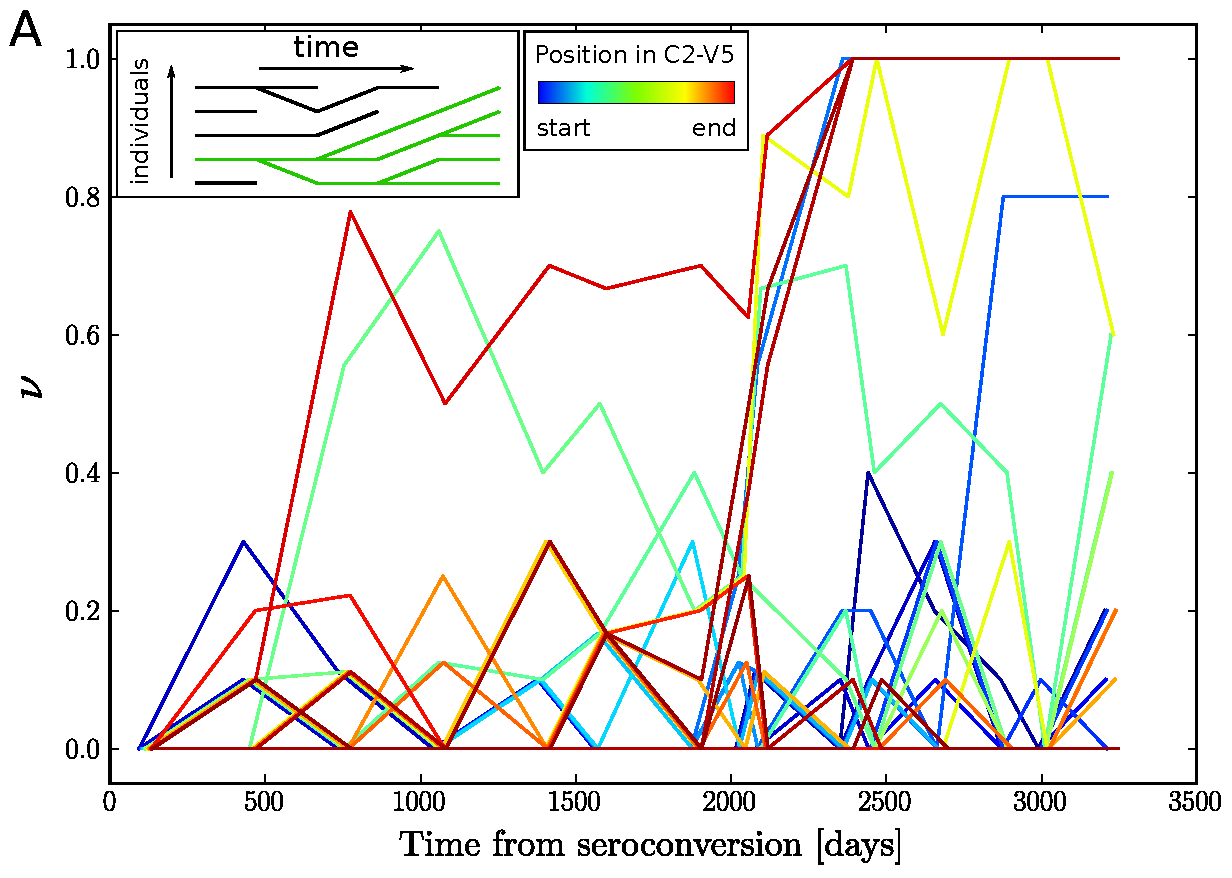
\includegraphics[width=\linewidth]{Shankarappa_allele_freqs_trajectories_syn_p1.pdf}
\label{fig:aftsyn}}\\
 \subfloat{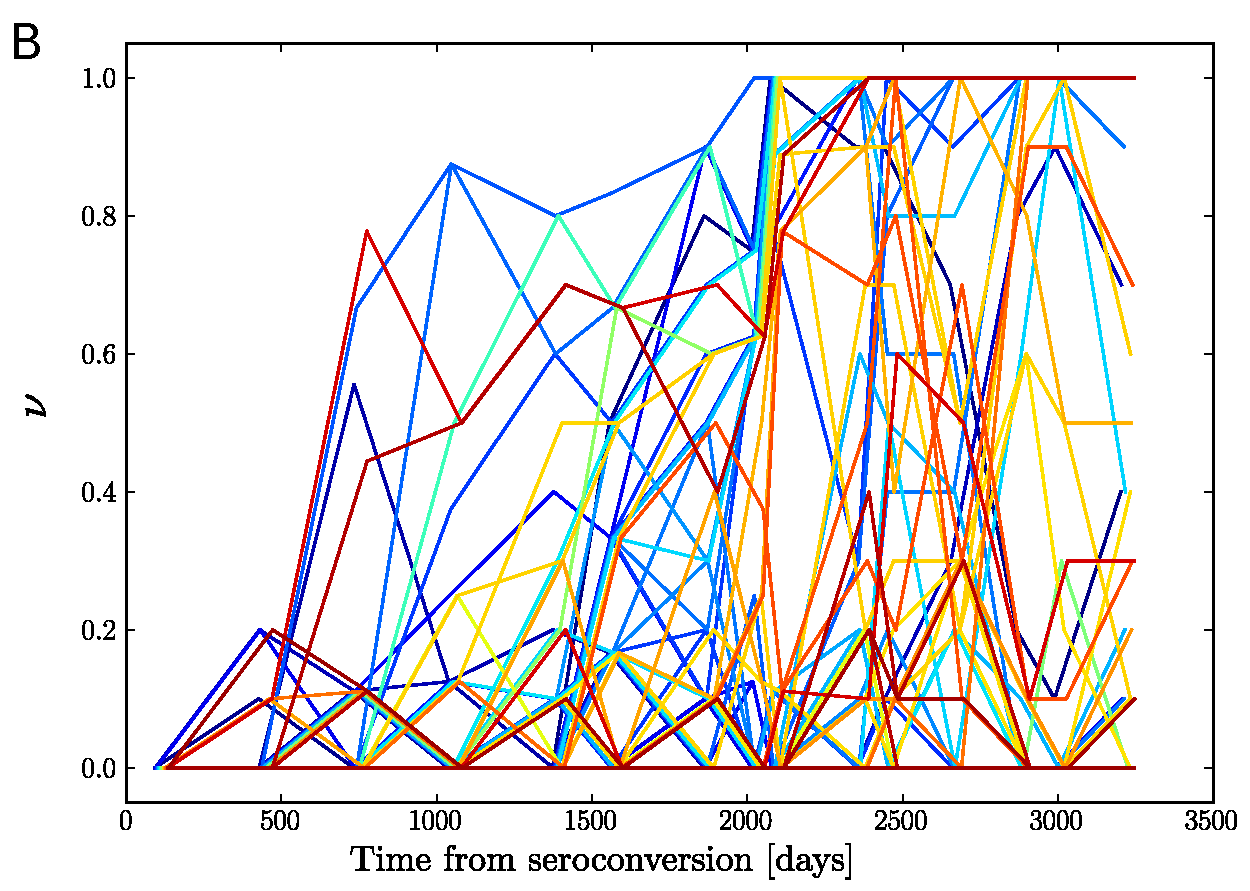
\includegraphics[width=\linewidth]{Shankarappa_allele_freqs_trajectories_nonsyn_p1.pdf}
\label{fig:aftnonsyn}}
\caption{Time series of allele frequencies in \env, C2-V5, from
patient 1~\cite{shankarappa_consistent_1999},
divided by synonymous (panel A) and nonsynonymous (panel B) derived alleles.
While nonsynonymous mutations frequently fix, very few synonymous
mutations do even though they are frequently observed at intermediate
frequencies. Colors indicate the position of the site along the C2-V5 region
(blue to red). Inset: the fixation probability $P_\text{fix}(\nu)$ of a neutral mutation
is simply the likelihood that the future common ancestor is currently carrying
it, i.e., its frequency $\nu$.}
\label{fig:aft}
\end{center}
\end{figure}

When interpreting these results for the fixation probabilities, it is important
to distinguish between random mutations and polymorphisms at a given frequency,
which have already been filtered by selection.
A polymorphism could be beneficial to the virus and on its way to fixation. In
this case, we expect that it fixes almost surely given we see it at high
frequency. If, on the other hand, the polymorphism is deleterious it must have
gotten to high frequency by chance (genetic drift or hitchhiking), and
we expect that selection will drive it out of the population again. Hence our
observations suggest that many of the synonymous polymorphisms at intermediate
frequencies in the part of \env~that includes the hypervariable regions are
deleterious, while outside this regions polymorphisms are mostly roughly
neutral. Note that this does not imply that all synonymous mutations are neutral
-- only those mutations observed at high frequencies, which have been
experiencing selection for some time already, tend to be neutral.

\begin{figure}
\begin{center}
\subfloat{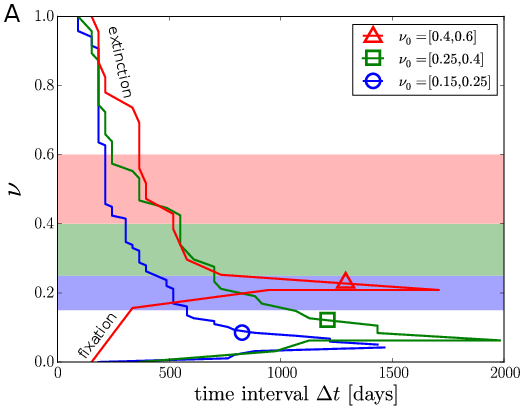
\includegraphics[width=0.9\linewidth]{fixation_times}
\label{fig:fixp1}}\\
\subfloat{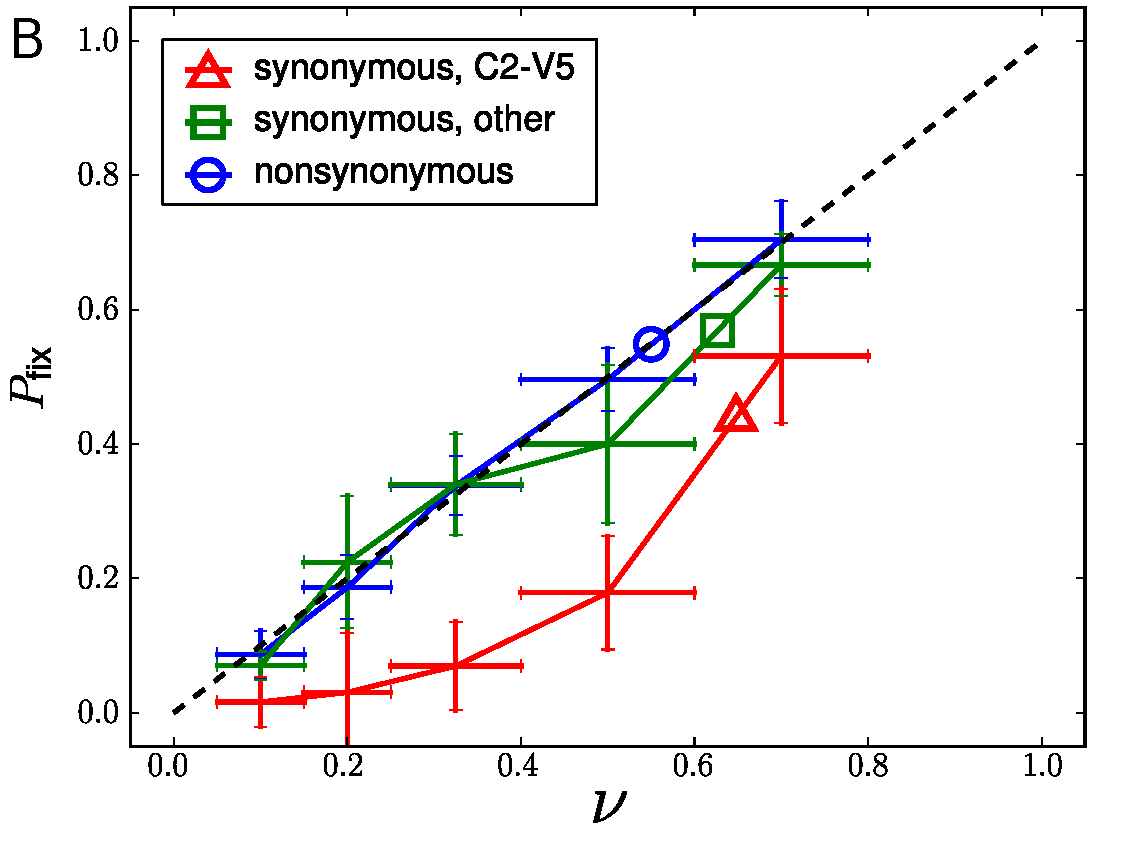
\includegraphics[width=0.9\linewidth]{fixation_probabilities}
\label{fig:fixp2}}
\caption{Fixation and loss of synonymous mutations.
Panel A) Time
course of loss and fixation of synonymous mutations observed in a frequency interval $\nu_0$. 
In each frequency interval, the  fraction of synonymous
mutations that ultimately fix is the fixation probability conditional on the
initial frequency.
Panel B) Fixation probability of derived synonymous
alleles as a function of $\nu_0$ in C2-V5 is below the neutral
expectation indicated by the diagonal line. This suppression is not
oberserved in other parts of {\it env} or for nonsynonymous mutations.
The horizontal error bars on the abscissa are bin sizes, the vertical ones the
standard deviation after 100 patient bootstraps of the data. Data from
Refs.~\cite{shankarappa_consistent_1999, bunnik_autologous_2008}.}
\label{fig:fixp}
\end{center}
\end{figure}

%%%%%%%%%%%%%%%%%%%%%%%%%%%%%%%%%%%%%%%%%%%%%%%%%%%%%%%%%%%%%%%%%%%%%%%%%
\subsection{Synonymous mutations in C2-V5 tend to disrupt conserved RNA stems}
%%%%%%%%%%%%%%%%%%%%%%%%%%%%%%%%%%%%%%%%%%%%%%%%%%%%%%%%%%%%%%%%%%%%%%%%%
One possible {\it a priori} explanation for lack of fixation of synonymous
mutations in C2-V5 are  secondary structures in the viral RNA. It has
been suggested early on that parts of the viral genome that has the potential to
form stems is better conserved than the
remainder~\citep{forsdyke_reciprocal_1995,snoeck_mapping_2011}.

Recently, the propensity of nucleotides of the HIV genome to form base pairs has
been measured using the SHAPE assay (a biochemical reaction preferentially
altering unpaired bases)~\citep{watts_architecture_2009}. The SHAPE assay has
shown that the variable regions V1 to V5 tend to be unpaired, while the
conserved regions between those variable regions form stems. We partition all
synonymous alleles observed at intermediate frequencies above 10-15\% depending
on their final destiny (fixation or extinction). Subsequently, we align our
sequences to the reference NL4-3 strain used in
ref.~\citep{watts_architecture_2009} and assign them SHAPE reactivities. As
shown in \FIG{SHAPEA}, the reactivities of fixed
alleles (red line) are systematically larger than of alleles are lost (blue
line) (Kolmogorov-Smirnov test, $P\approx 0.002$).
In other words, alleles that are likely to break RNA helices are also more
likely to revert and finally be lost from the population. As a control, the
average over non-observed but potentially available polymorphisms lies between
the two curves (green line), as expected (because only some of these mutations
would interfere with stem-loop formation).
To test the hypothesis that mutations in C2-V5 are lost because they break stems in the
conserved streches between the variable loops, we split the synonymous mutations in the
extended V1-V5 region further into conserved and variable regions and found that
the biggest depression in fixation probability is observed in the conserved
stems, while the variable loops show little deviation from the neutral
signature, see \FIG{SHAPEB}. This is consistent with important stem structures
in conservered regions between loops.

In addition to RNA secondary structure, we have considered other possible
explanations for a fitness defect of synonymous mutations, in particular codon
usage bias (CUB). HIV is known to prefer A-rich codons over highly expressed
human codons~\citep{jenkins_extent_2003,kuyl_biased_2012}. We do not find,
however, any evidence for a contribution of CUB to the ultimate fate of
synonymous alleles consistent with the fact that CUB between HIV and human genes
is not shrinking at the macroevolutionary level \citep{kuyl_biased_2012}. 
Furthermore, CUB in the V1-C5 region is not very different from other parts of
the HIV genome, whereas the reduced fixation probability is only observed there. In
conclusion, although we cannot exclude an effect of CUB on fitness as a general
rule, we expect it to be a minor effect in our context. 


\begin{figure}
\begin{center}
\subfloat{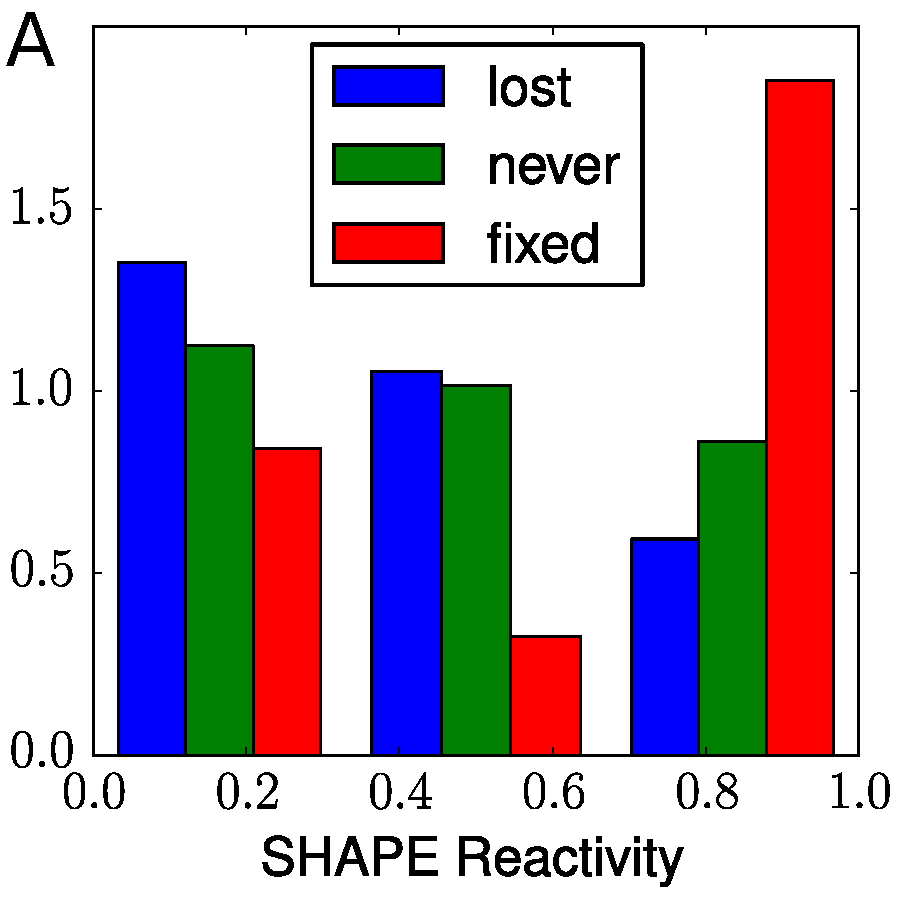
\includegraphics[height=0.46\linewidth]{reactivities_histograms_syn}
\label{fig:SHAPEA}}
\subfloat{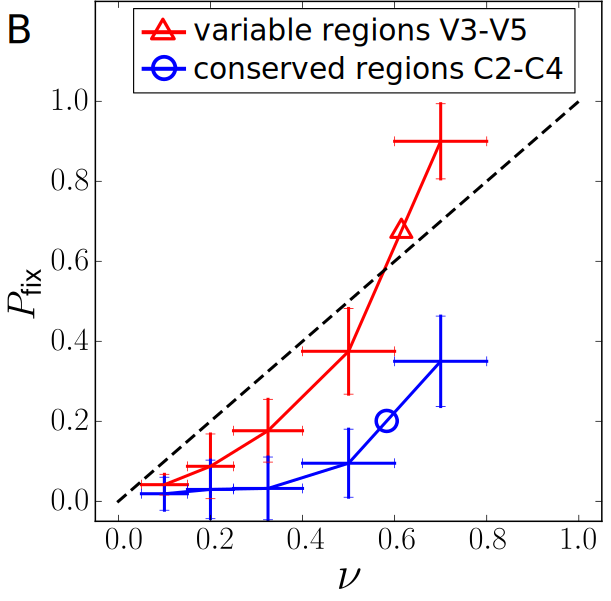
\includegraphics[height=0.46\linewidth]{fixation_probabilities_VnonV}\label{fig:SHAPEB}}
\caption{Permissible synonymous mutations have
high SHAPE reactivities.
Panel A) Synonymous substitions have
substantially higher SHAPE reactivities than mutations that reach frequencies above 15\%, but are
susequently lost (restricted to the vicinity of variable loops). This difference
is quantified by a cumulative histogram ($p=0.002$, Kolmogorov-Smirnov two 
sample test). Mutations that are never
observered show an intermediate distribution of SHAPE values.
Panel B) Fixation probability of synonymous mutations in C2-V5
separately for variable loops and the connecting conserved regions, that
harbor conserved RNA stems. As expected, fixation probability is lower inside
the conserved regions. Data from Refs.~\cite{shankarappa_consistent_1999,
bunnik_autologous_2008, liu_selection_2006}.}
\label{fig:SHAPE}
\end{center}
\end{figure}


%%%%%%%%%%%%%%%%%%%%%%%%%%%%%%%%%%%%%%%%%%%%%%%%%%%%%%%%%%%%%%%%%%%%%%%%%
\subsection{Deleterious mutations are brought to high frequency by hitchhiking}
%%%%%%%%%%%%%%%%%%%%%%%%%%%%%%%%%%%%%%%%%%%%%%%%%%%%%%%%%%%%%%%%%%%%%%%%%
While the observation that some fraction of synonymous mutations is deleterious
is not unexpected, it seems odd that we observe them at high population
frequency -- at least in some regions of the genome. The region of \env~ in
which we observe deleterious mutations at high frequency, however, is special in
that it undergoes frequent adaptive changes to evade recognition by neutralizing
antibodies~\cite{williamson_adaptation_2003,richman_rapid_2003}. Due to the limited amount of
recombination in HIV~\cite{neher_recombination_2010,batorsky_estimate_2011},
deleterious mutations that are linked to adaptive variants can reach high
frequency. This process is known as hitchhiking \citep{smith_hitch-hiking_1974}
or genetic draft \citep{gillespie_genetic_2000,neher_genetic_2011}.

The potential for hitchhiking is already apparent from the allele frequency
trajectories in \FIG{aft}, where many mutations appear to change rapidly in
frequency as a flock. In order
to be advected to high frequency by a linked adaptive mutation, the deleterious
effect of the mutation has to be substantially smaller than the adaptive effect.
The latter was estimated to be on the order of $s_a = 0.01$ per day~\citep{neher_recombination_2010}.
The approximate magnitude of the deleterious effects can be estimated from
\FIG{fixp1}, that shows the distribution of times for synonymous
alleles to reach the fix or get lost starting from intermediate frequencies. The
typical time to loss is of the order of 500 days. If this loss is driven by the
deleterious effect of the mutation, this corresponds to deleterious effects of
roughly $s_d \sim - 0.002$ per day.

\begin{figure}
\begin{center}
\subfloat{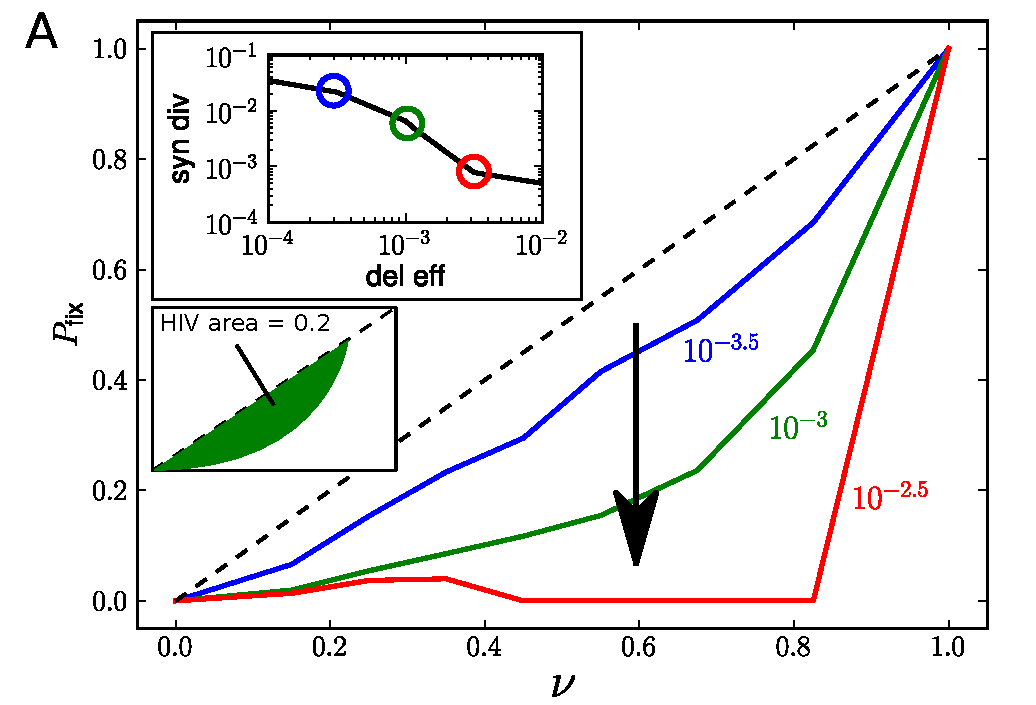
\includegraphics[width=\linewidth]{simulations_graduallydel.pdf}
\label{fig:simfixpvar}}\\
\subfloat{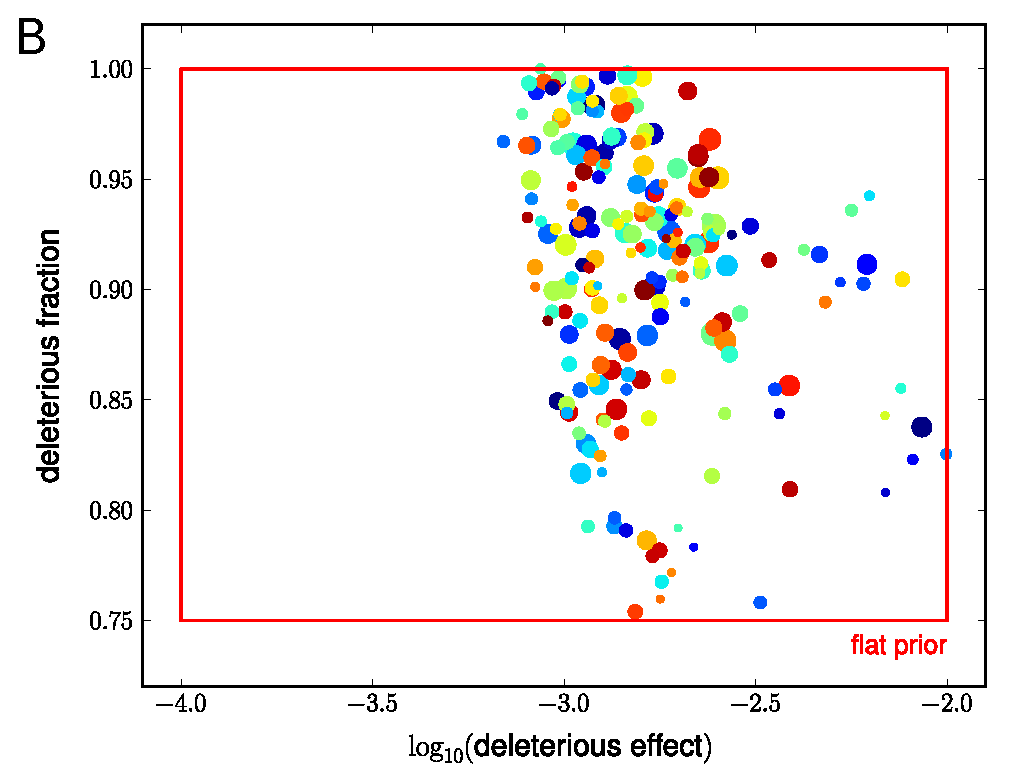
\includegraphics[width=\linewidth]{simulations_syn.pdf}
\label{fig:simsfig}}
\caption{Distribution of selection coefficients on synonymous sites. Panel A)
The depression in $P_\text{fix}$ depends on the deleterious effect size 
of the synonymous alleles. This parameter also reduces synonymous
diversity, measured by the probability of a derived allele to be found at
intermediate frequencies $P_\text{interm}$ (first inset).
Panel B) To assess the parameter space that affects synonymous fixation and
diversity, we run many simulations with random parameters for deleterious effect
size, fraction of deleterious synonymous sites, average size of escape
mutations (color, blue ($10^{-2.5}$) to red ($10^{-1.5}$)), and rate of
introduction of new epitopes (marker size, from $10^{-3}$ to $10^{-2}$ per
generation). Mostly simulations with small deleterious effects and relatively
high deleterious fractions of synonymous mutations reproduce synonymous HIV-like
fixation probability and diversity. Parameters are chosen uniformly on a
logarithmic scale from the indicated windows. This simulation assumes 6
roughly equivalent escape mutations per epitope; see supplement for alternative
models.}
\label{fig:simheat}
\end{center}
\end{figure}

To get a better idea of the range of parameters that are compatible with the
observations and our interpretation, we perform computer simulations of
evolving viral populations assuming a mix of positive and purifying selection
and rare recombination.
For this purpose, we use the simulation package FFPopSim, which includes a
module dedicated to intrapatient HIV evolution~\citep{zanini_ffpopsim:_2012}. 

The first result of the simulations is that genetic draft can indeed bring weakly
deleterious mutations to high frequencies and results in a dependence of the
fixation probability on initial frequency that is compatible with observations
(see \FIG{simfixpvar}).
To assess the reduction in fixation probability quantitatively, we calculate
the area between the measured fixation probability and the diagonal, which is
the neutral expectation (\FIG{simfixpvar}, lower inset). This area spans a range
between $-0.5$ (no fixation at all), zero (neutral-like curve), and $+0.5$ (always
fixed). Furthermore, we quantify synonymous diversity via the probability
$P_\text{interm}$ of a synonymous derived allele to be at intermediate frequencies
$0.25 < \nu < 0.75$ (\FIG{simfixpvar}, top inset).
The HIV data correspond to an area $A_\text{syn} \sim -0.2$  for synonymous
changes and $A_\text{nonsyn} \sim 0$ for nonsynonymous changes,
and a synonymous diversity $P_\text{interm} \sim 0.005$.
In the three simulations shown in \FIG{simfixpvar}, the fixation probability of
synonymous alleles decreases from the neutral expectation ($A_\text{syn} \sim 0$) to zero
($A_\text{syn} \sim -0.5$) as their fitness effect
worsens; the synonymous diversity plummets as well, as it is harder for
deleterious mutations to reach the frequency threshold of 0.25.

To map the parameter range of the model that is compatible with the data, we
repeatedly simulated the evolution with random choices for the deleterious
effect of synonymous mutations, the fraction of synonymous mutations that are
deleterious, the escape rate and the frequency of new escapes. Note that the
escape rate is sum of two factors: (a) the beneficial effect due to the ability to
evade the immune system minus (b) the fitness side costs in terms of structure,
stability, etc.
Among all simulations, we select the ones that show $A_\text{syn}$ and
$P_\text{interm}$ as observed in the data, i.e., a large depression in fixation
probability of synonymous mutations but, simulteneously, a moderately high
synonymous diversity. Specifically, \FIG{simsfig} shows parameter combinations
for which we found $A_\text{syn} < -0.15$ and $0.0025 < P_\text{interm} <
0.010$. This selection imposes a strong
constraint on the deleterious fraction and effect size (see \FIG{simsfig}).
A high fraction ($\gtrsim 0.8$) of only slightly deleterious synonymous sites,
with effect size $|s_d| \sim 0.002$, is required. This result fits well the
expectation based on the fixation/extinction times above (see \FIG{fixp1}).
The results are plausible:
(a) since high frequency bins are enriched in neutral mutations (it is easier
for them to hitchhike), a depression in $\pfix$ will be
visible only if deleterious mutations are pervasive; (b) in order to
hitchhike, the deleterious effect size has to be much smaller than the escape
rate, otherwise the
double mutant has little or no fitness advantage; (c) mutations with a 
deleterious effect weaker than approximately $0.001$ behave neutrally
consistent with the typical coalescent times observed in HIV.

As long as only features of synonymous mutations are filtered, as performed
above, no strong correlation of the two nonsynonymous parameters, escape rate
and rate of appearance of epitopes, is observed; in \FIG{simsfig}, the points
shown possess a variety of shapes and colors. In most of these simulations, 
however, nonsynonymous mutations almost always fix once they reach high frequencies
-- their nonsynonymous fixation area is well above zero. This is incompatible
with the blue line in \FIG{fixp}: in an HIV infection, nonsynonymous mutations fix as if they
were neutral. Although there are no doubts that nonsynonymous variation in the
variable regions is driven by positive selection and not by genetic drift, the
biological reason for the neutral-like curve in \FIG{fixp} is unclear.
Inspecting the trajectories of nonsynonymous mutations
suggests the rapid rise and fall of many alleles. We test two possible
mechanisms that are biologically plausible and could explain the transient rise
of nonsynonymous mutations: time-dependent selection and within-epitope
competition.

The former hypothesis can be formulated as follows: if the immune system
recognizes the escape mutant before its fixation, the mutant might cease to be
beneficial and disappear soon, despite its quick initial rise in frequency. In support of this idea,
\citet{richman_rapid_2003, bunnik_autologous_2008} report antibody responses to
escape mutants. These respones are delayed by a few months, roughly matching the
average time needed by an escape mutant to cross frequencies of order one.
In the alternative hypothesis, several different escape
mutations within the same epitope might arise almost simultaneously and start to
spread. Their benefits are not additive, because each of them is
essentially sufficient to escape. As a consequence, several escape mutations rise to
high frequency rapidly, while the one with the smallest cost in terms of replication,
packaging, etc.~is most likely to eventually fix. The emergence of
multiple sweeping nonsynonymous mutations in real HIV infections has been shown
previously~\citep{moore_limited_2009, bar_early_2012}.
We tested both hypotheses in our simulation framework and they both seem to
achieve a reduced, neutral-like fixation probability while maintaining a high
rate of substitutions, compatibly with HIV measurements (see supplementary
materials).
In real HIV infections, both mechanisms are likely to be playing a role, as they
are not mutually exclusive.

%%%%%%%%%%%%%%%%%%%%%%%%%%%%%%%%%%%%%%%%%%%%%%%%%%%%%%%%%%%%%%%%%%%%%%%%%
\section{Discussion}
%%%%%%%%%%%%%%%%%%%%%%%%%%%%%%%%%%%%%%%%%%%%%%%%%%%%%%%%%%%%%%%%%%%%%%%%%
Despite several known functional roles for RNA secondary structure in the HIV
genome, synonymous mutations are often used as approximately neutral markers in
evolutionary studies of viruses. By analyzing the fate of mutations in
longitudinal data of HIV \env{} evolution, we have shown that the majority of
synonymous mutations in the conserved regions C2-C5 of the \env~gene are deleterious.
Comparison with recent biochemical studies of binding propensity of bases in RNA
genome suggest that these mutations are deleterious, at least in part, because they disrupt
stems in RNA secondary structures. Furthermore, we provide evidence that these
mutations are brought to high frequency through linkage to adaptive mutations.

Contrary to na\"ive expectations, the adaptive escape mutations do not seem to be
unconditionally beneficial. Otherwise we would observe almost sure fixation of
nonsynonymous mutations once they reach intermediate frequencies. Instead, we
find that the fixation probability of nonsynonymous mutations is roughly given
by its frequency. There are several possible explanations for this observation. 
Similar to synonymous mutations, the majority of nonsynonymous mutations could
be weakly deleterious and the adaptive and deleterious parts conspire to yield
the neutral-like averaged fixation probability. We consider this possibility
inplausible since the amino-acid sequence outside the variable loops is much
more conserved that the synonymous positions, suggesting that the majority of
the nonsynonymous mutations is much more deleterious (see supplementary
materials). 

Alternatively, the lack of fixation could be due to (a) time dependent environment
through an immune system that is catching up, or (b) competition between mutations
that mediate escape within the same epitope. We explore both of these
possibilities and find that both produce the desired effect. Furthermore, there
is experimental evidence in support of both of these hypotheses. Serum from HIV infected
individuals tyically neutralizes the virus that dominated the population a few
(3-6) month ago \citep{richman_rapid_2003}. This suggests that escape mutations
cease to be beneficial after a few months and might revert if they come with a
fitness cost. Deep sequencing of regions of \env{} after antibody escape have
revealed multiple escape mutations in the same epitope
\citep{moore_limited_2009, bar_early_2012}. Presumably, each one of these
mutations is sufficient for escape but most combinations of them don't provide
any additional benefit to the virus. Hence only one mutation will spread and the
others will be driven out of the population although they transiently reach high
frequencies. The rapid emergence of multiple escape mutations in the same
epitope implies a large population size that explores all necessary point mutations rapidly. A
similar point has been made recently by Boltz {\it et al.} in the context of
preexisting drug resistance mutations~\citep{boltz_ultrasensitive_2012}. 

The observed hitchhiking highlights the importance of linkage due to infrequent
recombination for the evolution of HIV
\citep{neher_recombination_2010,batorsky_estimate_2011,
josefsson_majority_2011}. The recombination rate has been estimated to be on the
order of $\rho = 10^{-5}$ per base and day. It takes roughly $t_{sw} =
\epsilon^{-1} \log \nu_0$ generations for escape mutation with escape rate
$\epsilon$ to rise from an initially low frequency $\nu_0\sim \mu$ to frequency
one. This implies that a region of length $l = (\rho t_{sw})^{-1} = \epsilon /
\rho \log \nu_0$ remains linked to the adaptive mutation. With $\epsilon=0.01$,
we have $l\approx 100$ bases. Hence we expect strong linkage between the
variable loops and the intervening sequence, but none far beyond the variable
regions, consistent with the lack of signal outside of C1-V5. In case of much
stronger selection -- such as observed during early CTL escape or drug
resistance evolution -- the linked  region is of course much larger
\citep{nijhuis_stochastic_1998}.

A functional significance of the insulating RNA structure stems between the
hyper-variable loops has been proposed
previously~\citep{watts_architecture_2009, sanjuan_interplay_2011}.
Our analysis is limited by the availability of
longitudinal data which requires a focus on the the variable regions of \env.
Conserved RNA structures exist in different parts of the HIV genome (several are
known). In absence of repeated adaptive substitutions in the vicinity that cause
hitchhiking, the deleterious synonymous mutations remain at low frequencies and
can only be observed by deep sequencing methods. 

The fixation and extinction times and probabilities represent a rich and simple
summary statistics useful to characterize longitudinal sequence data and compare
to models via computer simulations.
A similar method has been recently used in a longitudinal study of
influenza~\citep{strelkowa_clonal_2012}. The propagators suggested in that
paper, however, represent ratios between nonsynonymous and synonymous mutations.
The latter is used as an approximately neutral control and this method can
therefore not be used to investigate synonymous changes themselves.

Our results emphasize the inadequacy of independent site
models of HIV evolution and the common assumption that selection is time
independent or additive. If genetic variation is only transiently beneficial,
existing methods to quantify selection will yield substantial underestimates
\citep{williamson_adaptation_2003,neher_rate_2010,batorsky_estimate_2011}.

%%%%%%%%%%%%%%%%%%%%%%%%%%%%%%%%%%%%%%%%%%%%%%%%%%%%%%%%%%%%%%%%%%%%%%%%%
\section{Methods}
%%%%%%%%%%%%%%%%%%%%%%%%%%%%%%%%%%%%%%%%%%%%%%%%%%%%%%%%%%%%%%%%%%%%%%%%%
\subsection{Sequence data collection}
%%%%%%%%%%%%%%%%%%%%%%%%%%%%%%%%%%%%%%%%%%%%%%%%%%%%%%%%%%%%%%%%%%%%%%%%%
Longitudinal intrapatient viral RNA sequences are collected for published
studies~\citep{shankarappa_consistent_1999, liu_selection_2006,
bunnik_autologous_2008} and downloaded from the Los Alamos National Laboratory
(LANL) HIV sequence database~\citep{LANL2012}. The sequences from some patients
show signs of HIV compartimentalization into subpopulations and are
discarded (see supplementary materials);
a total of 11 patients with approximately 6 time points each and 10
sequences per time point are eventually analyzed. The time interval or
resolution between two consecutive sequences is approximately 6 to 18 months.

%%%%%%%%%%%%%%%%%%%%%%%%%%%%%%%%%%%%%%%%%%%%%%%%%%%%%%%%%%%%%%%%%%%%%%%%%
\subsection{Sequence analysis}
%%%%%%%%%%%%%%%%%%%%%%%%%%%%%%%%%%%%%%%%%%%%%%%%%%%%%%%%%%%%%%%%%%%%%%%%%
The sequences are aligned within each patient
via the translated amino acid sequence, using
Muscle~\citep{edgar_muscle:_2004}, and to the NL4-3 reference sequence used
by \citet{watts_architecture_2009} in the SHAPE assay. Within each patient, a
consensus nucleotide sequence at the first time point is used to classify
alleles as ancestral or derived at all sites. Problematic sites that include large frequencies of gaps
are excluded from the analysis to avoid artefactual substitutions due to
alignment errors. Time series of allele frequencies are extracted from the
sequences.

The synonymity of a mutation is assigned if the rest of the codon was
in the ancestral state and using the standard genetic code. Cases where more
than one mutation within the codon is observed are discarded. Slightly
different criteria for synonymous/nonsynonymous discrimination yield similar
results.

%%%%%%%%%%%%%%%%%%%%%%%%%%%%%%%%%%%%%%%%%%%%%%%%%%%%%%%%%%%%%%%%%%%%%%%%%
\subsection{Fixation probability and secondary structure}
%%%%%%%%%%%%%%%%%%%%%%%%%%%%%%%%%%%%%%%%%%%%%%%%%%%%%%%%%%%%%%%%%%%%%%%%%
For the estimate of times to fixation/extinction, polymorphisms are
binned by frequency and the time to reaching the first boundary (fixation or
extinction) is stored. For the fixation probability, the long-time limit of the
resulting curves is used, excluding polymorphisms that arise late in the
clinical history (hence would have no time to reach either boundary).

For the correlation analysis with RNA secondary structure, the SHAPE scores are
downloaded from the journal website~\citep{watts_architecture_2009}. By virtue
of the alignment of the longitudinal sequences with the reference used by
\citet{watts_architecture_2009}, SHAPE reactivities are assigned to most sites.
Problematic assignments in indel-rich regions are excluded from the analysis.
In order to restrict the analysis to synonymous polymorphisms, a lower frequency
threshold of 0.15 was used (other thresholds yield the same results). Since
very few polymorphisms hitchhike beyond, say, a frequency of 0.5, this pool is
enriched for to-be-lost mutations; hence the ``lost" curve in \FIG{SHAPEA}
contains much more points than the ``fixed" one.

The V loops and flanking regions are identified manually starting from the
annotated reference HXB2 sequence from the LANL HIV database~\citep{LANL2012}. A
similar approach is used to label the C2-V5 region sequenced in
ref.~\citep{shankarappa_consistent_1999}.

%%%%%%%%%%%%%%%%%%%%%%%%%%%%%%%%%%%%%%%%%%%%%%%%%%%%%%%%%%%%%%%%%%%%%%%%%
\subsection{Computer simulations}
%%%%%%%%%%%%%%%%%%%%%%%%%%%%%%%%%%%%%%%%%%%%%%%%%%%%%%%%%%%%%%%%%%%%%%%%%
Simulations are performed using the recently published software
FFPopSim~\citep{zanini_ffpopsim:_2012}. Both full-length HIV genomes and
\env{}-only simulations are performed and yield comparable results. For each
set of parameters, approximately 100 simulation runs are averaged over. In each
run, a random fitness landscape with specified statistical properties (e.g.
density of beneficial sites, average deleterious effect of synonymous changes) is generated.

For the discussion of simulation parameters, the areas below or above the neutral
diagonal were estimated from the binned fixation probabilities using linear
interpolation between the bin centers. This measure is sufficiently precise for
our purposes.

%%%%%%%%%%%%%%%%%%%%%%%%%%%%%%%%%%%%%%%%%%%%%%%%%%%%%%%%%%%%%%%%%%%%%%%%%
\subsection{Methods availability}
%%%%%%%%%%%%%%%%%%%%%%%%%%%%%%%%%%%%%%%%%%%%%%%%%%%%%%%%%%%%%%%%%%%%%%%%%
All analysis scripts, as well as the sequence alignment used, are available for download.

%%%%%%%%%%%%%%%%%%%%%%%%%%%%%%%%%%%%%%%%%%%%%%%%%%%%%%%%%%%%%%%%%%%%%%%%%
\section*{Acknowledgements}
%%%%%%%%%%%%%%%%%%%%%%%%%%%%%%%%%%%%%%%%%%%%%%%%%%%%%%%%%%%%%%%%%%%%%%%%%
We are grateful for stimulating discussions with Jan Albert and Trevor Bedford.
This work is supported by the ERC starting grant HIVEVO 260686.

%%%%%%%%%%%%%%%%%%%%%%%%%%%%%%%%%%%%%%%%%%%%%%%%%%%%%%%%%%%%%%%%%%%%%%%%%
\bibliographystyle{natbib}
\bibliography{bib}
%%%%%%%%%%%%%%%%%%%%%%%%%%%%%%%%%%%%%%%%%%%%%%%%%%%%%%%%%%%%%%%%%%%%%%%%%
\end{document}
%%%%%%%%%%%%%%%%%%%%%%%%%%%%%%%%%%%%%%%%%%%%%%%%%%%%%%%%%%%%%%%%%%%%%%%%%

